\subsection{Connecting the Dissertation Manuscripts}
\label{subsec:connecting-the-dissertation-manuscripts}

This dissertation is organized around the manuscripts of~\autoref{fig:conn_papers}.

\begin{figure}[p]
\begin{subfigure}{\textwidth}
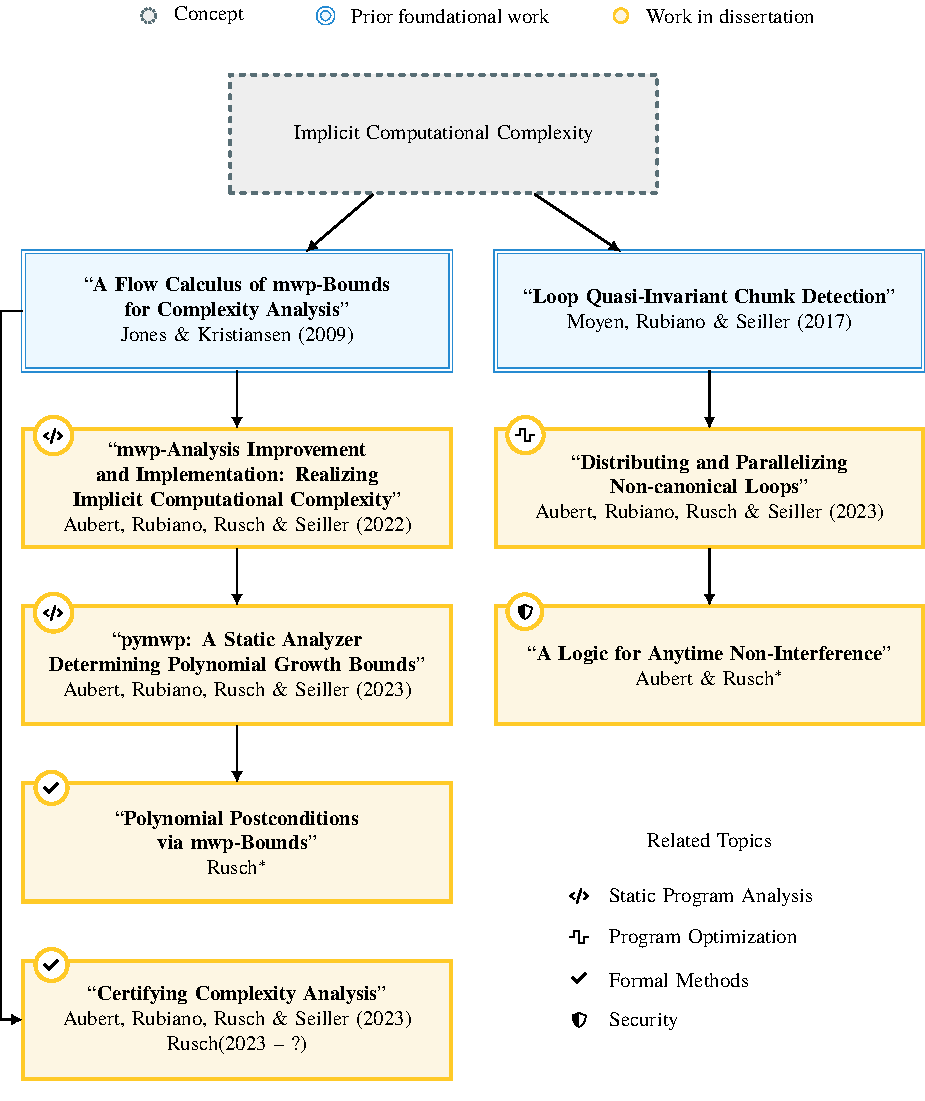
\includegraphics[width=\linewidth,keepaspectratio]{fig_conn_papers}
\end{subfigure}
\begin{center}
\resizebox{.85\textwidth}{!}{
\begin{subfigure}{\textwidth}{
\begin{tabularx}{\textwidth}{@{}X@{}cr@{}}
\toprule
\textbf{Title} & \textbf{Section} & \textbf{Background} \\
\midrule
{mwp-Analysis Improvement and Implementation\ldots}
& \aref{sec:fscd}
& \ref{icc}, \ref{static-analysis}, \ref{flow-calculus} \\
{Distributing and Parallelizing Non-canonical Loops}
& \ref{sec:vmcai}
& \ref{transforms} \\
{Polynomial Postconditions via mwp-Bounds}
& \ref{sec:postcond}
& \ref{flow-calculus}, \ref{verification} \\
{pymwp: A Static Analyzer Determining\ldots}
& \ref{sec:atva}, \aref{app:toolguide}
& \ref{icc}, \ref{static-analysis}, \ref{flow-calculus} \\
{A Logic for Anytime Non-Interference}
& \ref{sec:anytime}
& \ref{pl-sec} \\
{Certifying Complexity Analysis}
& \ref{coqpl}
& \ref{flow-calculus}, \ref{verification} \\
\bottomrule
\end{tabularx}}
\end{subfigure}}
\end{center}
\caption{Dissertation manuscripts.}
\label{fig:conn_papers}
\end{figure}

\subsection{Tips for Interacting With This Document}
\label{subsec:tips}

\subsubsection{Software Artifacts}\label{subsub:sw}
Each published and publication-ready manuscript in this dissertation, including the dissertation itself, comes with a corresponding software artifact.
A complete index of the artifacts is in~\aref{app:sec:artifacts}.
Each piece of software is archived for long-term retention, according to the long-term archival policies of the Association for Computing Machinery artifact guidelines~\cite{acm_badging}.
The software is achieved even if the venue of a manuscript did not arrange a formal artifact evaluation round.
Thus, each manuscript extends beyond the paper pages of this dissertation.

\subsubsection{Indices and Glossaries}

For convenience of the reader, this dissertation comes with three indices and glossaries\index{hello}\symbo{bigomega}.
The Term Index, in \autoref{sec:app:index}, lists technical terms and identifies where they are used in the dissertation.
The dissertation uses various acronyms where each acronym is defined at first-use.
To locate the long form afterward, refer to~\nameref{\acronymtype}.
A similar glossary is available for symbolic notations in the~\nameref{symbols}.

\subsubsection{Back-up Archival of External Documents}

The unpublished or miscellaneous external web pages and PDF files, that are referenced in the bibliography of this dissertation,
are pre-emptively archived on the Internet Archive with the Wayback Machine.
To recover a document from the Internet Archive, use the following format, substituting \pr|<URL>| by the document's URL\@.
\begin{center}
    \pr|https://web.archive.org/web/<URL>|
\end{center}
For example, the following URL may disappear in the future.
\begin{center}
    \url{https://types22.inria.fr/files/2022/06/TYPES_2022_paper_14.pdf}
\end{center}
In that case, the corresponding Internet Archive address produces the same document.
\begin{center}
    \url{https://web.archive.org/web/https://types22.inria.fr/files/2022/06/TYPES_2022_paper_14.pdf}
\end{center}

If a referenced external document was not readily available on the Internet even at the time of writing this dissertation,
the document is hosted and archived with the software deposit of this dissertation, \cf~\autoref{subsub:sw}.

\subsubsection{Line Numbers}
When referring to a specific line of source code,
we write \pr|L|, for \underline{L}ine;
followed by a natural number or numeric range that specifies the row(s) of interest.
For example, \pr|L3| means \enquote{line number 3}, and \pr|L10|--\pr|12| mean \enquote{lines 10 through 12}.
